\usetikzlibrary{arrows}
\usetikzlibrary{fit}

\tikzset{
	pics/conv/.style n args={5}{
		code = {
			\draw[draw=black] (#1, #2) rectangle ++ (1, 3) node[rotate=90, pos=0.5] {\large $#3 \times #4 \times #3$};
			\node[below] at (#1+0.5, #2+3.1) {\large #5};
		}
	},
	pics/text/.style n args={5}{
		code = {
			\draw[draw=black] (#1, #2) rectangle ++ (1, 3) node[rotate=#4, pos=0.5] {\huge #3};
			\node[below] at (#1+0.5, #2+3.1) {\large #5};
		}
	}
}

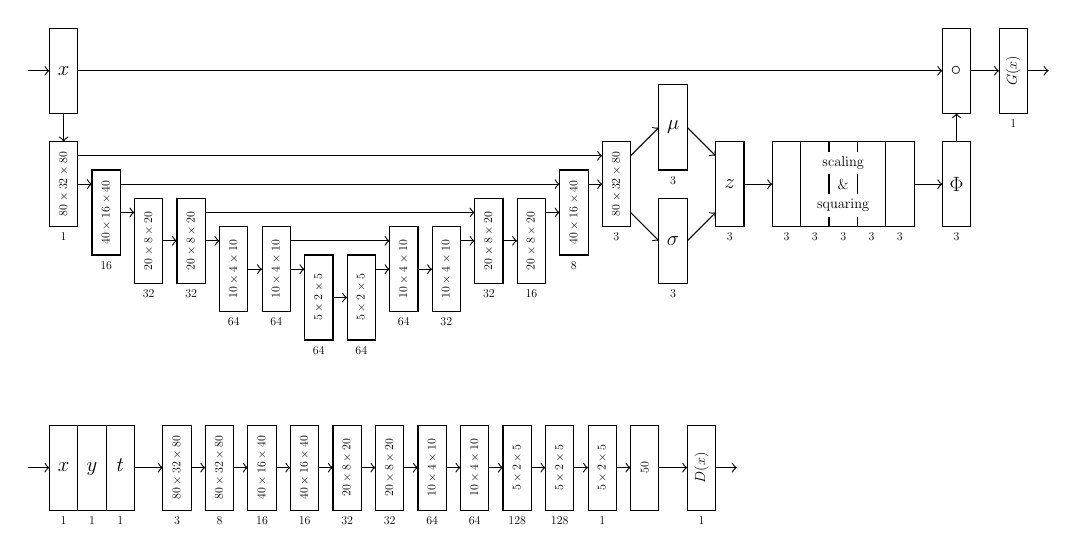
\begin{tikzpicture}[scale=0.36, line/.style={>=latex}, every node/.style={scale=0.36}, y=-1cm] 

	\pic{text={0}		{-4}	{$x$}	{0}	{}};

	\pic{conv={0}		{0}	{80}	{32}	{1}};
	\pic{conv={1.5}		{1}	{40}	{16}	{16}};
	\pic{conv={3}		{2}	{20}	{8}	{32}};
	\pic{conv={4.5}		{2}	{20}	{8}	{32}};
	\pic{conv={6}		{3}	{10}	{4}	{64}};
	\pic{conv={7.5}		{3}	{10}	{4}	{64}};
	\pic{conv={9}		{4}	{5}	{2}	{64}};
	\pic{conv={10.5}	{4}	{5}	{2}	{64}};
	\pic{conv={12}		{3}	{10}	{4}	{64}};
	\pic{conv={13.5}	{3}	{10}	{4}	{32}};
	\pic{conv={15}		{2}	{20}	{8}	{32}};
	\pic{conv={16.5}	{2}	{20}	{8}	{16}};
	\pic{conv={18}		{1}	{40}	{16}	{8}};
	\pic{conv={19.5}	{0}	{80}	{32}	{3}};
	
	\pic{text={21.5}	{-2}	{$\mu$}	{0}	{3}};
	\pic{text={21.5}	{2}	{$\sigma$}	{0}	{3}};
	
	\pic{text={23.5}	{0}	{$z$}	{0}	{3}};

	\pic{text={25.5}	{0}	{}	{0}	{3}};
	\pic{text={26.5}	{0}	{}	{0}	{3}};
	\pic{text={27.5}	{0}	{}	{0}	{3}};
	\pic{text={28.5}	{0}	{}	{0}	{3}};
	\pic{text={29.5}	{0}	{}	{0}	{3}};
	
    	\node [fill=white, inner sep=5pt] at (28, 0.75) {\Large scaling};
	\node [fill=white, inner sep=5pt] at (28, 1.5) {\Large \&};
    	\node [fill=white, inner sep=5pt] at (28, 2.25) {\Large squaring};

	\pic{text={31.5}	{0}	{$\Phi$}	{0}	{3}};
	
	\pic{text={31.5}	{-4}	{$\circ$}{90}	{}};
	
	\pic{text={33.5}	{-4}	{\Large $G(x)$}	{90}	{1}};

	\draw[->] (-0.75, -2.5) -- (0, -2.5);
	\draw[->] (0.5, -1) -- (0.5, 0);

	\draw[->] (1, 1.5) -- (1.5, 1.5);
	\draw[->] (2.5, 2.5) -- (3, 2.5);
	\draw[->] (4, 3.5) -- (4.5, 3.5);
	\draw[->] (5.5, 3.5) -- (6, 3.5);
	\draw[->] (7, 4.5) -- (7.5, 4.5);
	\draw[->] (8.5, 4.5) -- (9, 4.5);
	\draw[->] (10, 5.5) -- (10.5, 5.5);
	\draw[->] (11.5, 4.5) -- (12, 4.5);
	\draw[->] (13, 4.5) -- (13.5, 4.5);
	\draw[->] (14.5, 3.5) -- (15, 3.5);
	\draw[->] (16, 3.5) -- (16.5, 3.5);
	\draw[->] (17.5, 2.5) -- (18, 2.5);
	\draw[->] (19, 1.5) -- (19.5, 1.5);

	% distribution
	\draw[->] (20.5, 0.5) -- (21.5, -0.5);
	\draw[->] (20.5, 2.5) -- (21.5,  3.5);

	\draw[->] (22.5, -0.5) -- (23.5,  0.5);
	\draw[->] (22.5, 3.5) -- (23.5,  2.5);
	
	\draw[->] (24.5, 1.5) -- (25.5,  1.5);
	
	\draw[->] (30.5, 1.5) -- (31.5,  1.5);

	\draw[->] (32, 0) -- (32, -1);
	
	\draw[->] (1, -2.5) -- (31.5, -2.5);

	\draw[->] (32.5, -2.5) -- (33.5,  -2.5);
	\draw[->] (34.5, -2.5) -- (35.25, -2.5);

	% skip connections
	\draw[->] (1, 0.5) -- (19.5, 0.5);
	\draw[->] (2.5, 1.5) -- (18, 1.5);
	\draw[->] (5.5, 2.5) -- (15, 2.5);
	\draw[->] (8.5, 3.5) -- (12, 3.5);
	
	%\node [fill=white, inner sep=5pt] at (10.25, 2) {skip connections};

	% --- critic ---
	\pic{text={0}		{10}	{$x\vphantom{xyt}$}	{0}	{1}};
	\pic{text={1}		{10}	{$y\vphantom{xyt}$}	{0}	{1}};
	\pic{text={2}		{10}	{$t\vphantom{xyt}$}	{0}	{1}};

	\pic{conv={4}		{10}	{80}	{32}	{3}};
	\pic{conv={5.5}		{10}	{80}	{32}	{8}};
	\pic{conv={7.0}		{10}	{40}	{16}	{16}};
	\pic{conv={8.5}		{10}	{40}	{16}	{16}};
	\pic{conv={10.0}		{10}	{20}	{8}	{32}};
	\pic{conv={11.5}		{10}	{20}	{8}	{32}};
	\pic{conv={13.0}		{10}	{10}	{4}	{64}};
	\pic{conv={14.5}	{10}	{10}	{4}	{64}};
	\pic{conv={16}		{10}	{5}	{2}	{128}};
	\pic{conv={17.5}	{10}	{5}	{2}	{128}};
	
	\pic{conv={19}		{10}	{5}	{2}	{1}};
	
	\pic{text={20.5}	{10}	{\large $50$}	{90} {}};
	\pic{text={22.5}		{10}	{\Large $D(x)$}	{90} {1}};

	\draw[->] (-0.75, 11.5) -- (0, 11.5);
	\draw[->] (3, 11.5) -- (4, 11.5);

	\draw[->] (5, 11.5) -- (5.5, 11.5);
	\draw[->] (6.5, 11.5) -- (7, 11.5);
	\draw[->] (8, 11.5) -- (8.5, 11.5);
	\draw[->] (9.5, 11.5) -- (10, 11.5);
	\draw[->] (11, 11.5) -- (11.5, 11.5);
	\draw[->] (12.5, 11.5) -- (13, 11.5);
	\draw[->] (14, 11.5) -- (14.5, 11.5);
	\draw[->] (15.5, 11.5) -- (16, 11.5);
	\draw[->] (17, 11.5) -- (17.5, 11.5);
	\draw[->] (18.5, 11.5) -- (19, 11.5);
	\draw[->] (20, 11.5) -- (20.5, 11.5);
	
	\draw[->] (21.5, 11.5) -- (22.5, 11.5);
	\draw[->] (23.5, 11.5) -- (24.25, 11.5);


\end{tikzpicture}
